% ЕМТ 2023, V клас — точен LaTeX препис от официалните файлове в Klasirane.com.
% Условия: https://klasirane.com/api/competitions/EMT/All/2023/5%20%D0%BA%D0%BB/probs
% SHA-256 (условия): afb2e36e2c61239e303a7f533c080def0b09151965588137ad165c54cd910eeb
% Решения: https://klasirane.com/api/competitions/EMT/All/2023/5%20%D0%BA%D0%BB/sol
% SHA-256 (решения): ee212c5fa30d978c4cf891538fb0a3b9f7553f9a42351d559071af5beba05c9f
% Точковите оценки, правописът, формулировките и видимите печатни особености са запазени от източника.
% Фигурата е пикселно-точен изрез без редакция от вградения JPEG на официалния PDF с условията.

Задача 5.1. Произведението на три двуцифрени числа $a$, $b$ и $c$ е равно на най-голямото четирицифрено число, което е кратно на 45 и се записва с четири различни нечетни цифри.

а) Колко е сборът на числата $a$, $b$ и $c$?

б) Ако дробта $\dfrac ab$ е правилна и съкратима, кое число трябва да се прибави към числителя и знаменателя на дробта $\dfrac ac$, за да се получи дроб, равна на $\dfrac cb$?

Решение. а) (3 точки) Най-голямото четирицифрено число, което е кратно на 5 и на 9 и се записва с четири различни нечетни цифри, е 9315.

Тъй като $9315=3\cdot3\cdot3\cdot3\cdot5\cdot23$, единственият начин да се представи като произведение на двуцифрени числа е $9315=(3\cdot3\cdot3)\cdot(3\cdot5)\cdot23=27\cdot15\cdot23$.

Сборът на числата $a$, $b$ и $c$ е $15+23+27=65$.

б) (3 точки) Числата $a$, $b$ и $c$ са 15, 23 и 27 в някакъв ред. Дробта $\dfrac ab$ е правилна и съкратима само когато $a=15$, $b=27$. Следователно $c=23$.

Когато към числителя и знаменателя на дробта $\dfrac ac=\dfrac{15}{23}$ се прибави едно и също число, разликата между числителя и знаменателя ще се запази и ще е $23-15=8$.

В дробта $\dfrac cb=\dfrac{23}{27}$ разликата между числителя и знаменателя е $27-23=4$. Като я разширим с 2, ще получим $\dfrac{23}{27}=\dfrac{46}{54}$, като в $\dfrac{46}{54}$ разликата между числителя и знаменателя е 8.

Числото, което трябва да се прибави към числителя и знаменателя на дробта $\dfrac{15}{23}$, за да се получи $\dfrac{46}{54}$, е $46-15=54-23=31$.

Задача 5.2. Правоъгълникът $ABCD$ има обиколка 2464 cm и е сглобен от 19 квадрата, както е показано на чертежа.

a) Намерете дължината и широчината на правоъгълника $ABCD$.

б) Най-малко на колко еднакви квадрата може да се разреже правоъгълникът $ABCD$?

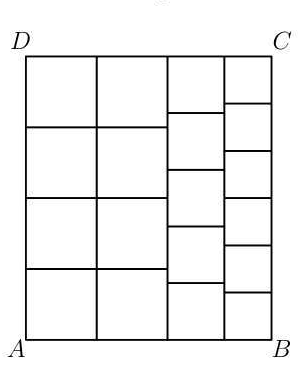
\includegraphics[max width=0.32\textwidth, alt={Правоъгълник ABCD, сглобен от 19 квадрата}, center]{assets/5-2-squares.png}

Решение. а) (3 точки) Страната $BC$ е разделена на 6, на 5 и на 4 равни отсечки. Тъй като $\operatorname{НОК}(6;5;4)=60$, да означим $BC=60x$.

Страната на най-големите квадрати е $(60x):4=15x$, страната на средните квадрати е $(60x):5=12x$, а страната на най-малките квадрати е $60x:6=10x$. Тогава $AB=2\cdot15x+12x+10x=52x$.

Обиколката на правоъгълника е $2464=2\cdot(60x+52x)$, откъдето $1232=112x$ и намираме $x=1232:112=11$.

Страните на правоъгълника са $AB=52\cdot11=572$ cm, $BC=60\cdot11=660$ cm.

б) (3 точки) Най-големите еднакви квадрати, с които може да се покрие правоъгълникът $ABCD$, имат страна, равна на $\operatorname{НОД}(572;660)=44$ cm. Техният брой е
$$
(572:44)\cdot(660:44)=13\cdot15=195.
$$

Задача 5.3. Професор Попов наблюдава през телескопа си галактика ЕМТ2023. В нея около звездата МАТ1 се въртят четири планети – Делимо, Делител, Частно и Остатък. Професорът забелязал, че на 18.11.2023 г. планетите са наредени в една линия. Той знае, че планетата Делимо прави пълна обиколка и се връща на същото място на всеки 3 земни дни, планетата Делител – на всеки 20 дни, планетата Частно – на всеки 60 дни, а планетата Остатък – на всеки 30 дни.

а) На коя дата четирите планети за пръв път ще са отново на първоначалните си места (от 18.11.2023 г.), подредени в една линия?

б) Професорът изчислил, че когато планетата Делимо направи $A$ пълни обиколки, планетата Делител направи $B$ пълни обиколки, планетата Частно направи $C$ пълни обиколки, а планетата Остатък направи $D$ пълни обиколки и отново застанат на първоначалните си места, то за пръв път броят на обиколките наистина ще са делимо, делител, частно и остатък, т.е. $A:B=C(\text{ост. }D)$. На коя дата ще стане това?

Решение. а) (3 точки) Четирите планети застават на първоначалните си места на всеки $\operatorname{НОК}(3,20,60,30)=60$ дни. Следователно за пръв път ще бъдат отново там 60 дни след 18.11.2023, на 17.01.2024 г.

б) (4 точки) Планетите ще бъдат на първоначалните си места след 60, 120, 180, 240, 300, 360 дни и т.н. Ще запишем в табличка колко обиколки е направила всяка от планетите за това време.

$$
\begin{array}{c|rrrrrr}
\text{Планета} & \multicolumn{6}{c}{\text{Брой обиколки}}\\
 & \text{за 60 дни} & \text{за 120 дни} & \text{за 180 дни} & \text{за 240 дни} & \text{за 300 дни} & \text{за 360 дни}\\ \hline
\text{Делимо} & 20 & 40 & 60 & 80 & 100 & 120\\
\text{Делител} & 3 & 6 & 9 & 12 & 15 & 18\\
\text{Частно} & 1 & 2 & 3 & 4 & 5 & 6\\
\text{Остатък} & 2 & 4 & 6 & 8 & 10 & 12
\end{array}
$$

С непосредствена проверка установяваме, че за пръв път условието е изпълнено след 360 дни, защото $120:18=6$ (ост.12). Това ще се случи 360 дни след 18.11.2023, на 12.11.2024 г. (отбележете, че 2024 година е високосна и това е 6 дни преди 18.11.2024 г.).

Задача 5.4. Дадени са четири различни естествени числа $a$, $b$, $c$ и $d$, за които са изпълнени условията:

• $\operatorname{НОК}(a;b)=\operatorname{НОК}(c;d)=2520$;

• $\operatorname{НОД}(a;b)=\operatorname{НОД}(c;d)=14$;

• числото $a$ има 3 пъти повече делители, отколкото числото $b$,

• числото $c$ има 3 пъти повече делители, отколкото числото $d$.

a) Намерете числата $a+c$ и $b+d$.

б) Колко числа, които не надхвърлят $a+c$, са взаимнопрости с $b+d$?

Решение. а) (3 точки) Тъй като $2520=2^3\cdot3^2\cdot5\cdot7$ и $14=2\cdot7$, числата с НОК 2520 и НОД 14 могат да са:

1. случай. $2\cdot7$ и $2^3\cdot3^2\cdot5\cdot7$. Но $2\cdot7$ има $2\cdot2=4$ делители, а $2^3\cdot3^2\cdot5\cdot7$ има $4\cdot3\cdot2\cdot2=48$ делители; това не са търсените числа.

2. случай. $2\cdot7\cdot3^2$ и $2^3\cdot5\cdot7$. Но $2\cdot7\cdot3^2$ има $2\cdot2\cdot3=12$ делители, а $2^3\cdot5\cdot7$ има $4\cdot2\cdot2=16$ делители; това не са търсените числа.

3. случай. $2\cdot7\cdot5$ и $2^3\cdot3^2\cdot7$. В този случай $2\cdot7\cdot5$ има $2\cdot2\cdot2=8$ делители, а $2^3\cdot3^2\cdot7$ има $4\cdot3\cdot2=24$ делители – 3 пъти повече от 8.

4. случай. $2\cdot7\cdot3^2\cdot5$ и $2^3\cdot7$. В този случай $2^3\cdot7$ има $4\cdot2=8$ делители, a $2\cdot7\cdot3^2\cdot5$ има $2\cdot2\cdot3\cdot2=24$ делители – 3 пъти повече от 8.

Следователно $a+c=2^3\cdot3^2\cdot7+2\cdot7\cdot3^2\cdot5=504+630=1134$ и $b+d=2\cdot5\cdot7+2^3\cdot7=70+56=126$.

б) (4 точки) Тъй като $b+d=126=2\cdot7\cdot3^2$, взаимнопростите със 126 числа не се делят нито на 2, нито на 3, нито на 7.

Измежду естествените числа от 1 до 1134 търсим тези, които не се делят нито на 2, нито на 3, нито на 7.

Измежду естествените числа от 1 до 1134 има:

$1134:2=567$ четни;

$1134:3=378$ кратни на 3;

$1134:7=162$ кратни на 7;

$1134:\operatorname{НОК}(2;3)=1134:6=189$ кратни на 2 и на 3;

$1134:\operatorname{НОК}(2;7)=1134:14=81$ кратни на 2 и на 7;

$1134:\operatorname{НОК}(3;7)=1134:21=54$ кратни на 3 и на 7;

$1134:\operatorname{НОК}(2;3;7)=1134:42=27$ кратни на 2, на 3 и на 7.

Следователно броят на числата от 1 до 1134, които се делят на 2, 3 или 7, е
$$
567+378+162-(189+81+54)+27=810;
$$
откъдето броят на числата от 1 до 1134, които не се делят нито на 2, нито на 3, нито на 7, е
$$
1134-810=324.
$$
